\documentclass[11pt]{article}

\usepackage{fullpage}
\usepackage{graphicx}
\usepackage{amsmath}
\usepackage{amssymb}
\usepackage{amsthm}
\usepackage{fancyvrb}

\parindent0in
\pagestyle{plain}
\thispagestyle{plain}

\newcommand{\myname}{Mehshan Mustafa}
\newcommand{\dated}{\today}

\newenvironment{theorem}[2][Theorem]{\begin{trivlist}
\item[\hskip \labelsep {\bfseries #1}\hskip \labelsep {\bfseries #2.}]}{\end{trivlist}}
\newenvironment{lemma}[2][Lemma]{\begin{trivlist}
\item[\hskip \labelsep {\bfseries #1}\hskip \labelsep {\bfseries #2.}]}{\end{trivlist}}
\newenvironment{exercise}[2][Exercise]{\begin{trivlist}
\item[\hskip \labelsep {\bfseries #1}\hskip \labelsep {\bfseries #2.}]}{\end{trivlist}}
\newenvironment{problem}[2][Problem]{\begin{trivlist}
\item[\hskip \labelsep {\bfseries #1}\hskip \labelsep {\bfseries #2.}]}{\end{trivlist}}
\newenvironment{question}[2][Question]{\begin{trivlist}
\item[\hskip \labelsep {\bfseries #1}\hskip \labelsep {\bfseries #2.}]}{\end{trivlist}}
\newenvironment{corollary}[2][Corollary]{\begin{trivlist}
\item[\hskip \labelsep {\bfseries #1}\hskip \labelsep {\bfseries #2.}]}{\end{trivlist}}
\newenvironment{solution}{\begin{proof}[Solution]}{\end{proof}}
\newenvironment{idea}[2][Proof Idea.]{\textit{#1} #2}

\begin{document}

\textbf{Introduction to the Theory of
Computation}\hfill\textbf{\myname}\\[0.01in]
\textbf{Chapter 1: Reqular Languages}\hfill\textbf{\dated}\\
\smallskip\hrule\bigskip

\begin{problem}{1.65}
Prove that for each $n > 0$, a language $B_{n}$ exists where
\end{problem}

\begin{problem}[Part]{a}
$B_{n}$ is recognizable by an NFA that has $n$ states.
\end{problem}

\begin{proof}
Let $\Sigma$ be any nonempty set of symbols. Define $B_{n}$ to be the language:
\[
B_{n} = \{w \ | \ w \ has \ length \ at \ least \ n-1 \}
\]
\begin{center}
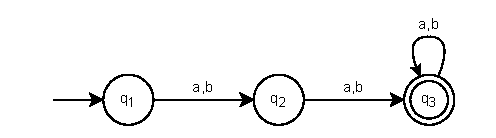
\includegraphics[scale=1.0]{Figures/Problem1.65.pdf} \\
Example of an NFA that recognizes $B_{3}$, where $\Sigma = \{a, b\}$.
\end{center}
$ $ \\
Construct the NFA $N=(Q, \Sigma, \delta, q_{0}, F)$ to recognize $B_{n}$:
\begin{enumerate}
\item $Q = \{q_{1}, \ q_{2}, \ \cdots, \ q_{n}\}$
\item $q_{0} = q_{1}$
\item $F = \{q_{n}\}$
\item Define $\delta(q_{i}, a)$ so that for any $q_{i} \in Q$ and any $a \in \Sigma$:
\begin{center}
$\displaystyle \delta(q_{i},\ a) \ =\begin{cases}
\{q_{i+1}\} & i < n \\
\{q_{n}\} & i = n \\
\end{cases} \ \ $
\end{center}
\end{enumerate}
\end{proof}

\begin{problem}[Part]{b}
If $B_{n} = A_{1} \cup \cdots \cup A_{k}$, for regular languages $A_{i}$, then at least one of the $A_{i}$ requires a DFA with exponentially many states.
\end{problem}

\begin{proof}
Solution Replace this text with the details of your proof or solution.
\end{proof}

\end{document}